\begin{problem}
  Show that $Q \implies S$, $R \implies T$, $\vdash$ $(Q \lor R) \implies (S
  \lor T)$.
\end{problem}

\begin{probsolution}
  \begin{table}[H]
    \begin{tabular}{lll}
      1. & $Q \implies S$ & Hypothesis \\
      2. & $R \implies T$ & Hypothesis \\
      3. & Assume $Q \lor R$ & Dischargeable Hypothesis \\
      4. & Case 1: $Q$ is true \\
      5. & $S$ & MP, for 4, for 1 \\
      6. & $S \lor T$ \\
      7. & Case 2: $R$ is true \\
      8. & $T$ & MP, for 7, for 2 \\
      9. & $S \lor T$ \\
      10. & $(Q \lor R) \implies (S \lor T)$ & DT, from 3 [3 - 9 unusable] \\
    \end{tabular}
  \end{table}
\end{probsolution}

\newpage

\begin{problem}
  Show that $(Q \land \neg T) \implies (Y \lor \neg P)$, $Y \implies (V \lor
  \neg X)$ $\vdash$ $(P \land X) \implies [Q \implies (T \lor V)]$.
\end{problem}

\begin{probsolution}
  \begin{table}[H]
    \begin{tabular}{lll}
      1. & $(Q \land \neg T) \implies (Y \lor \neg P)$ & Hypothesis \\
      2. & $Y \implies (V \lor \neg X)$ & Hypothesis \\
      3. & Assume $P \land X$ & Dischargeable Hypothesis \\
      4. & Assume $Q$ & Dischargeable Hypothesis \\
      5. & $P$ & LCS for 3 \\
      6. & $\neg (Q \land \neg T)$ & MT, for 5, for 1 \\
      7. & $\neg (Q \land \neg T) \iff \neg Q \lor T$ & Tautology \\
      8. & $\neg Q \lor T$ & MPB, for 6, for 7 \\
      9. & $T$ & DI, for 4, for 8 \\
      10. & $T \lor V$ \\
      11. & $Q \implies (T \lor V)$ & DT, from 4 [4 - 10 unusable] \\
      12. & $(P \land X) \implies [Q \implies (T \lor V)]$ & DT, from 3 [3 - 11 unusable] \\
    \end{tabular}
  \end{table}
\end{probsolution}

\newpage

\begin{problem}
  Give a line proof that $(A \subseteq X \land B \subseteq X) \implies (A \cup B
  \subseteq X)$.
\end{problem}

\begin{probsolution}
  \begin{table}[H]
    \begin{tabular}{ll}
      1. & Assume $A \subseteq X \land B \subseteq X$. \\
      2. & Since $A \subseteq X$, then $(\forall x \in A)[x \in X]$. \\
      3. & Since $B \subseteq X$, then $(\forall x \in B)[x \in X]$. \\
      4. & Then, if $x \in A$ or $x \in B$, then $x \in X$. \\
      5. & Therefore, $x \in A \cup B \implies x \in X$. \\
    \end{tabular}
  \end{table}
\end{probsolution}

\newpage

\begin{problem}
  Give a line proof that $(X \subseteq A \land X \subseteq B) \implies (X
  \subseteq A \cap B)$.
\end{problem}

\begin{probsolution}
  \begin{table}[H]
    \begin{tabular}{ll}
      1. & Assume $X \subseteq A \land X \subseteq B$. \\
      2. & Since $X \subseteq A$, then $(\forall x \in X)[x \in A]$. \\
      3. & Since $X \subseteq B$, then $(\forall x \in X)[x \in B]$. \\
      4. & Then, if $x \in X$, then $x \in A$ and $x \in B$. \\
      5. & Then, $x \in A \cap B$. \\
      6. & Therefore, $X \subseteq A \cap B$. \\
    \end{tabular}
  \end{table}
\end{probsolution}

\newpage

\begin{problem}
  Prove or disprove: If $a, b \in \N$ and $a \leq b$ then $M_a \subseteq M_b$.
\end{problem}

\begin{probsolution}
  The statement is false. For example, $a = 2$ and $b = 3$. Then $M_2 = \{1, 2,
  4, 6, 8, \dots\}$ and $M_3 = \{1, 3, 6, 9, 12, \dots\}$. But, $x = 2 \notin
  M_3$. Therefore, $M_a \not\subseteq M_b$.
\end{probsolution}

\newpage

\begin{problem}
  Prove or disprove: $M_4 \cap M_6 = M_{24}$.
\end{problem}

\begin{probsolution}
  \begin{table}[H]
    \begin{tabular}{ll}
      1. & $M_4$ is the set of all multiples of $4$. \\
      2. & $M_6$ is the set of all multiples of $6$. \\
      3. & lcm$(4, 6) = 12$. \\
      4. & Therefore, $M_4 \cap M_6$ is the set of all multiples of $12$. \\
      5. & Clearly, every multiple of $24$ is a multiple of $12$. \\
      6. & So, $M_{24} \subseteq M_4 \cap M_6$. \\
      7. & However, $M_4 \cap M_6$ includes all multiples of $12$, not just multiples of $24$. \\
      8. & For example, $12 \in M_4 \cap M_6$ but $12 \notin M_{24}$. \\
      9. & This means that $M_4 \cap M_6 \not\subseteq M_{24}$. \\
      10. & Therefore, $M_{24} \subseteq M_4 \cap M_6$. \\
    \end{tabular}
  \end{table}
\end{probsolution}

\newpage

\begin{problem}
  Prove or disprove: $M_4 \cap M_9 = M_{36}$.
\end{problem}

\begin{probsolution}
  \begin{table}[H]
    \begin{tabular}{ll}
      1. & $M_4$ is the set of all multiples of $4$. \\
      2. & $M_9$ is the set of all multiples of $9$. \\
      3. & lcm$(4, 9) = 36$. \\
      4. & Therefore, $M_4 \cap M_9$ is the set of all multiples of $36$. \\
      5. & So, $M_{36} \subseteq M_4 \cap M_9$. \\
      6. & $M_{36}$ is the set of all multiples of $36$. \\
      7. & Clearly, every multiple of $36$ is a multiple of $4$ and $9$. \\
      8. & So, $M_{36} \subseteq M_4$ and $M_{36} \subseteq M_9$. \\
      9. & Then, $M_{36} \subseteq M_4 \cap M_9$. \\
      10. & Therefore, $M_{36} = M_4 \cap M_9$. \\
    \end{tabular}
  \end{table}
\end{probsolution}

\newpage

\begin{problem}
  Give a line proof that $A \cup (B \cap C) = (A \cup B) \cap (A \cup C)$.
\end{problem}

\begin{probsolution}
  \begin{table}[H]
    \begin{tabular}{ll}
      1. & Assume $x \in A \cup (B \cap C)$. \\
      2. & Then, $x \in A \lor (x \in B \land x \in C)$. \\
      3. & If $x \in A$, then $x \in A \cup B$ and $x \in A \cup C$. \\
      4. & If $x \in B$ and $x \in C$, then $x \in A \cup B$ and $x \in A \cup C$. \\
      5. & Then, $x \in (A \cup B) \cap (A \cup C)$. \\
      6. & Therefore, $A \cup (B \cap C) \subseteq (A \cup B) \cap (A \cup C)$. \\
      7. & Assume $x \in (A \cup B) \cap (A \cup C)$. \\
      8. & Then, $x \in A \cup B$ and $x \in A \cup C$. \\
      9. & If $x \in A$, then $x \in A \cup (B \cap C)$. \\
      10. & If $x \notin A$ and $x \in B$ and $x \in C$, then $x \in A \cup (B \cap C)$. \\
      11. & Then, $x \in A \cup (B \cap C)$. \\
      12. & Therefore, $(A \cup B) \cap (A \cup C) \subseteq A \cup (B \cap C)$. \\
      13. & Therefore, $A \cup (B \cap C) = (A \cup B) \cap (A \cup C)$. \\
    \end{tabular}
  \end{table}
\end{probsolution}

\newpage

\begin{problem}
  Give a line proof showing that $X - (A \cup B) = (X - A) \cap (X - B)$, for
  all sets $A$, $B$, and $X$.
\end{problem}

\begin{probsolution}
  \begin{table}[H]
    \begin{tabular}{ll}
      1. & Assume $x \in X - (A \cup B)$. \\
      2. & Then, $x \in X$ and $x \notin A \cup B$. \\
      3. & Then, $x \in X$ and $x \notin A$ and $x \notin B$. \\
      4. & Then, $x \in X - A$ and $x \in X - B$. \\
      5. & Then, $x \in (X - A) \cap (X - B)$. \\
      6. & Therefore, $X - (A \cup B) \subseteq (X - A) \cap (X - B)$. \\
      7. & Assume $x \in (X - A) \cap (X - B)$. \\
      8. & Then, $x \in X - A$ and $x \in X - B$. \\
      9. & Then, $x \in X$ and $x \notin A$ and $x \notin B$. \\
      10. & Then, $x \in X$ and $x \notin A \cup B$. \\
      11. & Then, $x \in X - (A \cup B)$. \\
      12. & Therefore, $(X - A) \cap (X - B) \subseteq X - (A \cup B)$. \\
      13. & Therefore, $X - (A \cup B) = (X - A) \cap (X - B)$. \\
    \end{tabular}
  \end{table}
\end{probsolution}

\newpage

\begin{problem}
  Give a line proof showing that $X - (A \cap B) = (X - A) \cup (X - B)$, for
  all sets $A$, $B$, and $X$.
\end{problem}

\begin{probsolution}
  \begin{table}[H]
    \begin{tabular}{ll}
      1. & Assume $x \in X - (A \cap B)$. \\
      2. & Then, $x \in X$ and $x \notin A \cap B$. \\
      3. & Then, $x \in X$ and $x \notin A$ or $x \notin B$. \\
      4. & Then, $x \in X - A$ or $x \in X - B$. \\
      5. & Then, $x \in (X - A) \cup (X - B)$. \\
      6. & Therefore, $X - (A \cap B) \subseteq (X - A) \cup (X - B)$. \\
      7. & Assume $x \in (X - A) \cup (X - B)$. \\
      8. & Then, $x \in X - A$ or $x \in X - B$. \\
      9. & Then, $x \in X$ and $x \notin A$ or $x \notin B$. \\
      10. & Then, $x \in X$ and $x \notin A \cap B$. \\
      11. & Then, $x \in X - (A \cap B)$. \\
      12. & Therefore, $(X - A) \cup (X - B) \subseteq X - (A \cap B)$. \\
      13. & Therefore, $X - (A \cap B) = (X - A) \cup (X - B)$. \\
    \end{tabular}
  \end{table}
\end{probsolution}

\newpage

\begin{problem}
  If $f$ is a function from $S$ to $T$ and $A \subseteq S$, define $f(A) = \{x \mid (\exists y \in A)[x = f(y)]\}$. This is called the image of $A$ under $f$.

  \begin{enumerate}
    \item Give an example of a function $f : \N \to \N$ where
      $f(M_3 \cap \N) = \N$.

    \item Suppose $f : S \to T$ and $A \subseteq S$, $B \subseteq S$.
      \begin{enumerate}
        \item Prove that $f(A \cup B) = f(A) \cup f(B)$

        \item Prove that  $f(A \cap B) \subseteq f(A) \cap f(B)$

        \item Give an example of sets $S$, $T$, $A$, $B$, and a function $f$ for which $f(A) \cap f(B) \not\subseteq f(A \cap B)$. [Hint: Start by trying to prove that $f(A) \cap f(B) \subseteq f(A \cap B)$, and see where you get stuck.]
      \end{enumerate}
  \end{enumerate}
\end{problem}

\begin{probsolution}
  \begin{enumerate}
    \item Let $f : \N \to \N$ be defined by $f(x) = \sfrac{n}{3}$. Then, $f(M_3
      \cap \N) = \N$. With this definition, for any $m \in \N$, there exists a
      multiple of 3, specifically $3m$, such that $f(3m) = m$. Therefore, $f(M_3
      \cap \N) = \N$.

    \item Suppose $f : S \to T$ and $A \subseteq S$, $B \subseteq S$.
      \begin{enumerate}
        \item Here's the line proof for $f(A \cup B) = f(A) \cup f(B)$.

          \hspace*{-0.5em}\begin{tabular}{ll}
            1. & Assume $x \in f(A \cup B)$. \\
            2. & Then, $x = f(y)$ for some $y \in A \cup B$. \\
            3. & Then, $y \in A$ or $y \in B$. \\
            4. & Then, $x = f(y) \in f(A)$ or $x = f(y) \in f(B)$. \\
            5. & Then, $x \in f(A) \cup f(B)$. \\
            6. & Therefore, $f(A \cup B) \subseteq f(A) \cup f(B)$. \\
            7. & Assume $x \in f(A) \cup f(B)$. \\
            8. & Then, $x \in f(A)$ or $x \in f(B)$. \\
            9. & Then, $x = f(y)$ for some $y \in A$ or $y \in B$. \\
            10. & Then, $y \in A \cup B$. \\
            11. & Then, $x = f(y) \in f(A \cup B)$. \\
            12. & Therefore, $f(A) \cup f(B) \subseteq f(A \cup B)$. \\
            13. & Therefore, $f(A \cup B) = f(A) \cup f(B)$. \\
          \end{tabular}

        \item Here's the line proof for $f(A \cap B) \subseteq f(A) \cap f(B)$.

          \hspace*{-0.5em}\begin{tabular}{ll}
            1. & Assume $x \in f(A \cap B)$. \\
            2. & Then, $x = f(y)$ for some $y \in A \cap B$. \\
            3. & Then, $y \in A$ and $y \in B$. \\
            4. & Then, $x = f(y) \in f(A)$ and $x = f(y) \in f(B)$. \\
            5. & Then, $x \in f(A) \cap f(B)$. \\
            6. & Therefore, $f(A \cap B) \subseteq f(A) \cap f(B)$. \\
          \end{tabular}

        \item Let $S = \{1, 2\}$, $T = \{0, 1\}$, $A = \{1\}$, and $B = \{2\}$.
          Define $f : S \to T$ by $f(1) = 0$ and $f(2) = 0$. Then $f(A) =
          \{f(1)\} = \{0\}$, $f(B) = \{f(2)\} = \{0\}$, $f(A) \cap f(B) =
          \{0\}$, but $A \cap B = \emptyset$. So, $f(A) \cap f(B) = \emptyset
          \not\subseteq f(A \cap B) = \{0\}$.
      \end{enumerate}
  \end{enumerate}
\end{probsolution}

\newpage

\begin{problem}
  Yoda has a bunch of eggs, and you have to figure out how many.
  \begin{enumerate}
    \item He tells you two facts: When you separate the eggs into groups of 11,
      there are 3 left over. When you separate the eggs into groups of 8, there
      are 4 left over.

      Given these facts, what is the least number of eggs that Yoda could have?

    \item Suppose Yoda also tells you that he has between  100 and 200 eggs.
      Given this additional piece of information, you can determine exactly how
      many eggs Yoda has. How many?

    \item The next day Yoda comes back with a lot more eggs. This time he says:
      When I separate the eggs into groups of 11, there are 3 left over. When I
      separate them into groups of 300, there are 51 left over. What is the
      least number of eggs that Yoda could have?
  \end{enumerate}
\end{problem}

\begin{probsolution}
  \begin{enumerate}
    \item We need to find the smallest positive integer $n$ such that:
      \begin{align*}
        n &\equiv_{11} 3 \\
        n &\equiv_8 4
      \end{align*}

      From $n \equiv_{11} 3$, we can write $n = 11k + 3$ for some integer
      $k$. Substituting $n = 11k +3 $ into $n \equiv_8 4$
      \[%
        11k + 3 \equiv_8 4 \implies 11k \equiv_8 1
      .\]%
      Since $11 \equiv_8 3$, we have
      \[%
        3k \equiv_8 1
      .\]%

      To solve $3k \equiv_8 1$, we need to find an integer $k$ such that $3k$
      gives a remainder of 1 when divided by 8. If $k = 3$, then $3 \cdot 3 = 9
      \equiv_8 1$. So $k = 3$ is a solution, giving us
      \[%
        n = 11k + 3 = 11 \cdot 3 + 3 = 36
      .\]%
      Thus, the smallest positive integer $n$ that satisfies both conditions is
      $36$.

    \item Since we know from $(i)$ that $n = 36$ is a solution, any solution can
      be written in the form
      \[%
        n = 36 + 88m
      ,\]%
      where $88$ is the least common multiple of 11 and 8, and $m$ is an
      integer.

      Now, we need $n$ to be between 100 and 200
      \[%
        100 \leq 36 + 88m \leq 200 \implies 0.727 \leq m \leq 1.864
      .\]%
      Since $m$ is an integer, the only possible value for $m$ is $m = 1$,
      giving us
      \[%
        n = 36 + 88 \cdot 1 = 124
      .\]%

      So, with the additional information, the exact number of eggs Yoda has is
      $124$.

    \item Now Yoda has more eggs and gives us new conditions
      \begin{align*}
        n &\equiv_{11} 3 \\
        n &\equiv_{300} 51
      \end{align*}

      From $n \equiv_{300} 51$, we can write $n = 300k + 51$ for some integer
      $k$. Substitute $n = 300k + 51$ into $n \equiv_{11} 3$
      \[%
        300k + 51 \equiv 3 \pmod{11}
      .\]%
      Since $300 \equiv_{11} 3$ and $51 \equiv_{11} 7$, we have
      \[%
        3k + 7 \equiv_{11} 3 \implies 3k \equiv_{11} -4 \implies 3k \equiv_{11} 7
      .\]%

      To solve $3k \equiv_{11} 7$, we need to find an integer $k$ such that $3k$
      gives a remainder of 7 when divided by 11. If $k = 9$, then $3 \cdot 9 =
      27 \equiv_{11} 7 \pmod{11}$. So $k = 9$ is a solution. This gives us
      \[%
        n = 300k + 51 = 300 \cdot 9 + 51 = 2751
      .\]%
      The smallest number of eggs that Yoda could have is $2751$.
  \end{enumerate}
\end{probsolution}

\newpage

\begin{problem}
  You have a huge collection of $1 \times 2$ dominoes (or tiles), and a $2
  \times 11$ checkerboard:

  \tikzstyle{int}=[draw, fill=blue!20, rectangle, minimum height=1em, 
  minimum width=4em]
  \begin{center}
    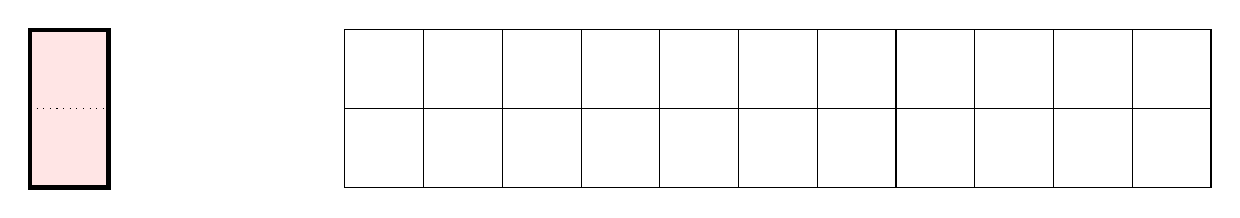
\begin{tikzpicture}[node distance=0.5cm]
      \filldraw[fill=red!10,ultra thick] (0,0) rectangle (1,2);
      \draw [dotted] (0,1) to (1,1);
      \draw (4,0) rectangle (15,2);
      \draw (4,1) to (15,1);
      \draw (5,0) to (5,2);
      \draw (6,0) to (6,2);
      \draw (7,0) to (7,2);
      \draw (8,0) to (8,2);
      \draw (9,0) to (9,2);
      \draw (10,0) to (10,2);
      \draw (11,0) to (11,2);
      \draw (12,0) to (12,2);
      \draw (13,0) to (13,2);
      \draw (14,0) to (14,2);
      \draw (15,0) to (15,2);
    \end{tikzpicture}
  \end{center}

  Your goal in this problem is to determine how many different ways there are to
  tile the checkerboard using your dominoes.

  To solve this problem, it is best to solve some smaller versions first. Let
  $S_n$ denote the number of different ways to tile a $2 \times n$ checkerboard.
  For example, $S_3 = 3$ as we see below:

  \begin{center}
    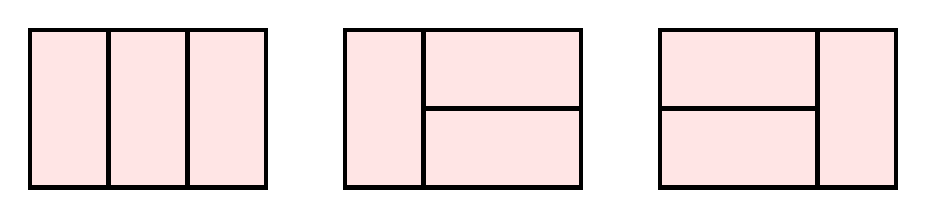
\begin{tikzpicture}[node distance=0.5cm]
      \filldraw[fill=red!10,ultra thick] (0,0) rectangle (1,2);
      \filldraw[fill=red!10,ultra thick] (1,0) rectangle (2,2);
      \filldraw[fill=red!10,ultra thick] (2,0) rectangle (3,2);
      \filldraw[fill=red!10,ultra thick] (4,0) rectangle (5,2);
      \filldraw[fill=red!10,ultra thick] (5,0) rectangle (7,1);
      \filldraw[fill=red!10,ultra thick] (5,1) rectangle (7,2);
      \filldraw[fill=red!10,ultra thick] (8,0) rectangle (10,1);
      \filldraw[fill=red!10,ultra thick] (8,1) rectangle (10,2);
      \filldraw[fill=red!10,ultra thick] (10,0) rectangle (11,2);
    \end{tikzpicture}
  \end{center}

  Make a table showing the values of $S_n$ for $1\leq n \leq 11$. As you are
  doing this, try to find a systematic way of finding all the tilings. Note any
  patterns that you find, and see if you can explain them. As a check, you
  should get $S_6=13$.
\end{problem}

\begin{probsolution}
  To solve the problem, let $S_n$ represent the number of ways to tile a $2
  \times n$ checkerboard with $1 \times 2$ dominoes.

  We start by analyzing smaller cases to build a table of values for $S_n$ and
  look for patterns.

  \begin{enumerate}
    \item For $n = 1$:
      \begin{enumerate}
        \item We can only place one domino vertically, so $S_1 = 1$.
      \end{enumerate}

    \item For $n = 2$:
      \begin{enumerate}
        \item We can either place two dominoes vertically or two horizontally,
          giving two possible configurations. So, $S_2 = 2$.
      \end{enumerate}

    \item For $n = 3$: We can either:
      \begin{enumerate}
        \item Place three vertical dominoes, or

        \item Place two horizontal dominoes on the bottom row and one vertical
          domino on top, or

        \item Place one vertical domino on the left and two horizontal dominoes
          on the right.
      \end{enumerate}

      Therefore, $S_3 = 3$.

    \item For $n = 4$: We can use:
      \begin{enumerate}
        \item Four vertical dominoes,

        \item Two horizontal pairs stacked, 

        \item Two vertical dominoes on the left and two horizontal on the right,
          or

        \item Two horizontal dominoes on top and two vertical on the bottom.
      \end{enumerate}

      So, $S_4 = 5$.
  \end{enumerate}

  By examining these small cases, we observe that to cover a $2 \times n$ board, we can either
  \begin{enumerate}
    \item Place one vertical domino at the left end, leaving a $2 \times (n-1)$
      board to cover, or

    \item Place two horizontal dominoes at the left end, leaving a $2 \times
      (n-2)$ board.
  \end{enumerate}

  This leads to the recurrence relation:
  \[%
    S_n = S_{n-1} + S_{n-2}
  .\]%
  with initial conditions $S_1 = 1$ and $S_2 = 2$. This relation is identical to
  the Fibonacci sequence shifted by one index.

  Using this recurrence, we can compute values up to $S_{11}$:

  \begin{center}
    \begin{tabular}{|c|c|c|c|c|c|c|c|c|c|c|c|}
      \hline
      $n$ & 1 & 2 & 3 & 4 & 5 & 6 & 7 & 8 & 9 & 10 & 11 \\
      \hline
      $S_n$ & 1 & 2 & 3 & 5 & 8 & 13 & 21 & 34 & 55 & 89 & 144 \\
      \hline
    \end{tabular}
  \end{center}

  Therefore, the number of ways to tile a $2 \times 11$ checkerboard is $S_{11}
  = 144$.
\end{probsolution}

\newpage

\begin{problem}
  A certain puzzle has three pegs, the leftmost peg starting out with a tower of $n$ disks. The object of the puzzle is to move this tower to the rightmost peg. The rules are that you can only move one disk at a time, the disk has to be moved from one peg to another, and you can never place a larger disk on top of a smaller disk. The following picture shows the starting position of the puzzle when $n = 4$:

  \begin{center}
    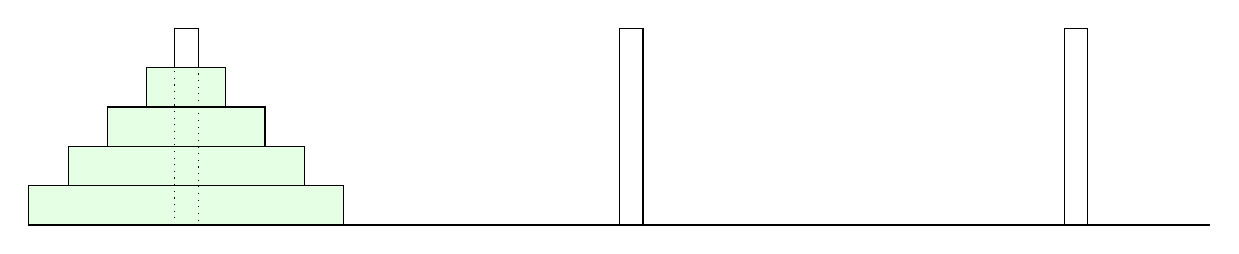
\begin{tikzpicture}[scale=0.5]
      \filldraw[fill=green!10]  (0,0) rectangle (8,1);
      \filldraw[fill=green!10]  (1,1) rectangle (7,2);
      \filldraw[fill=green!10]  (2,2) rectangle (6,3);
      \filldraw[fill=green!10]  (3,3) rectangle (5,4);
      \draw [dotted] (3.7,0) rectangle (4.3,5);
      \draw (3.7,4) rectangle (4.3,5);
      \draw (15,0) rectangle (15.6,5);
      \draw (26.3,0) rectangle (26.9,5);
      \draw [thick] (0,0) to (30,0);
    \end{tikzpicture}
  \end{center}

  Your goal in this problem is to determine the minimum number of moves needed to solve the puzzle when there are $11$ disks. Approach this in a similar way to what we did in problem \#13, by making a table showing the minimum number of moves to solve the $n$-disk game for $1 \leq n \leq 11$.
\end{problem}

\begin{probsolution}
  Let $M(n)$ represent the minimum number of moves required to solve the puzzle
  with $n$ disks. To understand this, we analyze smaller cases and observe the
  recursive pattern.

  \begin{enumerate}
    \item For $n = 1$: We can move the single disk directly to the target peg in
      one move. Thus, $M(1) = 1$.

    \item For $n = 2$: Move the first disk to an intermediate peg, the second
      disk to the target peg, and then the first disk from the intermediate peg
      to the target peg. Therefore, $M(2) = 3$.

    \item For $n = 3$: Move the first two disks to the intermediate peg (using
      $M(2) = 3$ moves), the third disk to the target peg, and then the two
      disks from the intermediate peg to the target peg (again using $M(2) = 3$
      moves). This gives $M(3) = M(2) + 1 + M(2) = 7$.
  \end{enumerate}

  By following this pattern, we observe that to solve the $n$-disk problem, we need to:
  \begin{enumerate}
    \item Move the top $n-1$ disks to an intermediate peg (requiring $M(n-1)$
      moves),

    \item Move the $n$-th disk to the target peg (1 move), and

    \item Move the $n-1$ disks from the intermediate peg to the target peg
      (again requiring $M(n-1)$ moves).
  \end{enumerate}

  This leads to the recurrence relation:
  \[%
    M(n) = 2M(n-1) + 1
  ,\]%
  with the initial condition $M(1) = 1$.

  Using this recurrence, we can calculate $M(n)$ for $1 \leq n \leq 11$:
  \begin{center}
    \begin{tabular}{|c|c|c|c|c|c|c|c|c|c|c|c|}
      \hline
      $n$ & 1 & 2 & 3 & 4 & 5 & 6 & 7 & 8 & 9 & 10 & 11 \\
      \hline
      $S_n$ & 1 & 3 & 7 & 15 & 31 & 63 & 127 & 255 & 511 & 1023 & 2047 \\
      \hline
    \end{tabular}
  \end{center}

  Thus, the minimum number of moves required to solve the Tower of Hanoi puzzle
  with 11 disks is $M(11) = 2047$.
\end{probsolution}
